Interfejs graficzny jest tworzony przez Django. Django na podstawie szablonów w postaci plików html oraz danych otrzymanych z funkcji napisanych w python'ie przygotowuje kompletny podgląd strony. 
Strona główna (Rysunek \ref{fig:stronaStartowa}) składa się z 3 dużych przycisków animowanych przy użyciu javascript, które doprowadzają do kolejnych zakładek. W górnej części strony znajdują się przyciski (''Indeks'', ''Podgląd stacji pogodowych'', ''Prognoza'', \textit{''Wczytaj dane''}, ''Autorzy''). W przypadku przycisku ''Wczytaj dane'' nie pojawi się on jeśli użytkownik jest niezalogowany. \newline 
\begin{figure}[p]
	\centering
	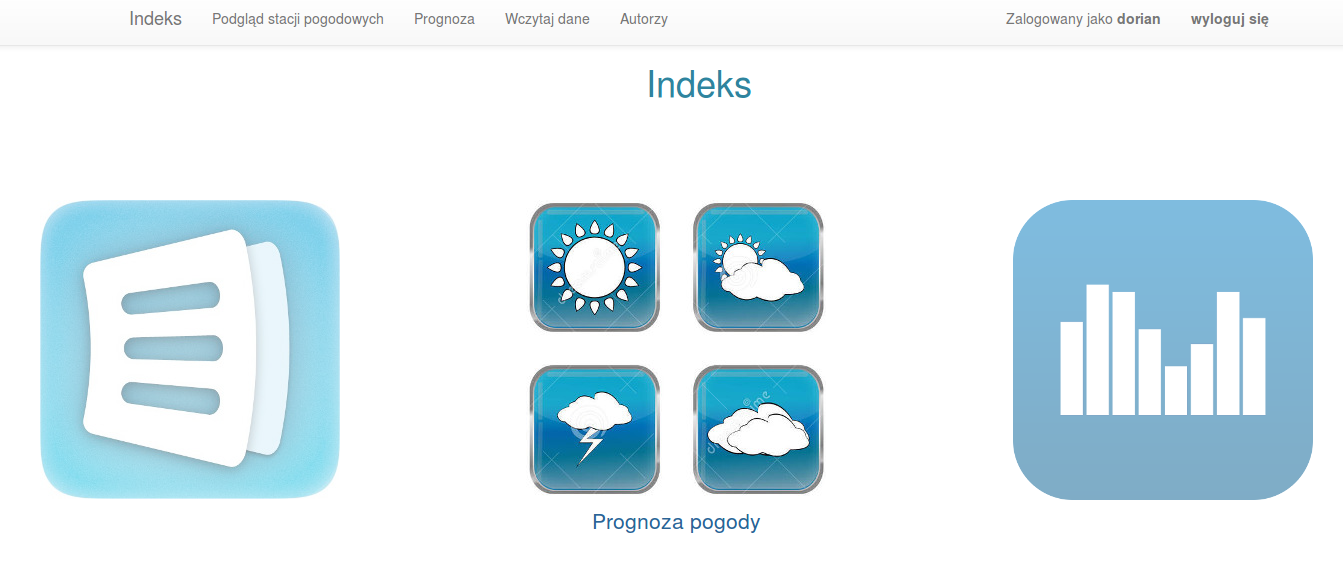
\includegraphics[width=\textheight, angle=90]{000}
	\caption{Strona startowa}
	\label{fig:stronaStartowa}
	\end{figure}

Po kliknięciu na zakładki ''Podgląd stacji pogodowych'' oraz ''Prognoza'' otwiera się bardzo podobna podstrona (Rysunek \ref{fig:podgladStacji}), która służy do wyboru rodzaju pomiaru oraz stacji, dla której dane mają zostać wyrysowane. W przypadku zalogowanych użytkowników pojawia się również możliwość skasowania danych w postaci przycisku ''delete''. 
\newline
\begin{figure}[p]
	\centering
	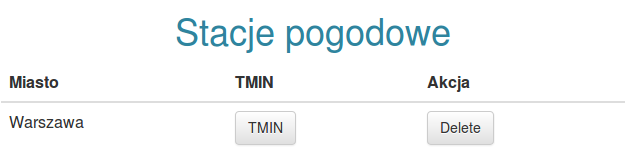
\includegraphics[width=\linewidth]{001}
	\caption{Podgląd stacji pogodowych - użytkownik zalogowany}
	\label{fig:podgladStacji}
	\end{figure}

Wykresy rysowane są przy użyciu biblioteki matplotlib (Rysunek \ref{fig:wykres}). 
\newline
\begin{figure}[p]
	\centering
	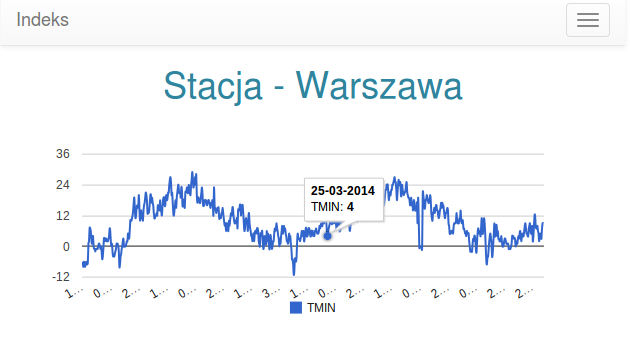
\includegraphics[width=\linewidth]{002}
	\caption{Wyrysowany wykres}
	\label{fig:wykres}
	\end{figure}

